% $Id: board2.tex 9464 2021-10-14 16:51:12Z mskala $

%
% MSK 014 Board 2 build instructions
% Copyright (C) 2022  Matthew Skala
%
% This program is free software: you can redistribute it and/or modify
% it under the terms of the GNU General Public License as published by
% the Free Software Foundation, version 3.
%
% This program is distributed in the hope that it will be useful,
% but WITHOUT ANY WARRANTY; without even the implied warranty of
% MERCHANTABILITY or FITNESS FOR A PARTICULAR PURPOSE.  See the
% GNU General Public License for more details.
%
% You should have received a copy of the GNU General Public License
% along with this program.  If not, see <http://www.gnu.org/licenses/>.
%
% Matthew Skala
% https://northcoastsynthesis.com/
% mskala@northcoastsynthesis.com
%

\chapter{Building Board 2}

The recommended order for building this module is to assemble Board 2, the
one further from the front panel, first.  That will make it easier to get
all the physical positioning right for the components that bridge between
the boards or pass through the panel.

Note that although I'm describing a separate step for each component value,
and that's how I built my prototype so as to have plenty of photo
opportunities, if you are reasonably confident about your skills you may
find it easier to populate all or most of the board (i.e.\ put the
components in place) and then solder them in a single step.  Except where
noted, the order in which you add components does not matter much.

The digital ICs on this board are sensitive to static electricity.  Although
they are not \emph{extremely} delicate, it would be appropriate to take
precautions like working on an anti-static surface and wearing a grounding
strap.

\section{Preliminaries}

Count out the right number of everything according to the bill of materials. 
There is an abbreviated BOM for Board~2, excluding a few items that will be
added when combining this board with Board~1, in Table~\ref{tab:b2bom}.

\nopagebreak
\noindent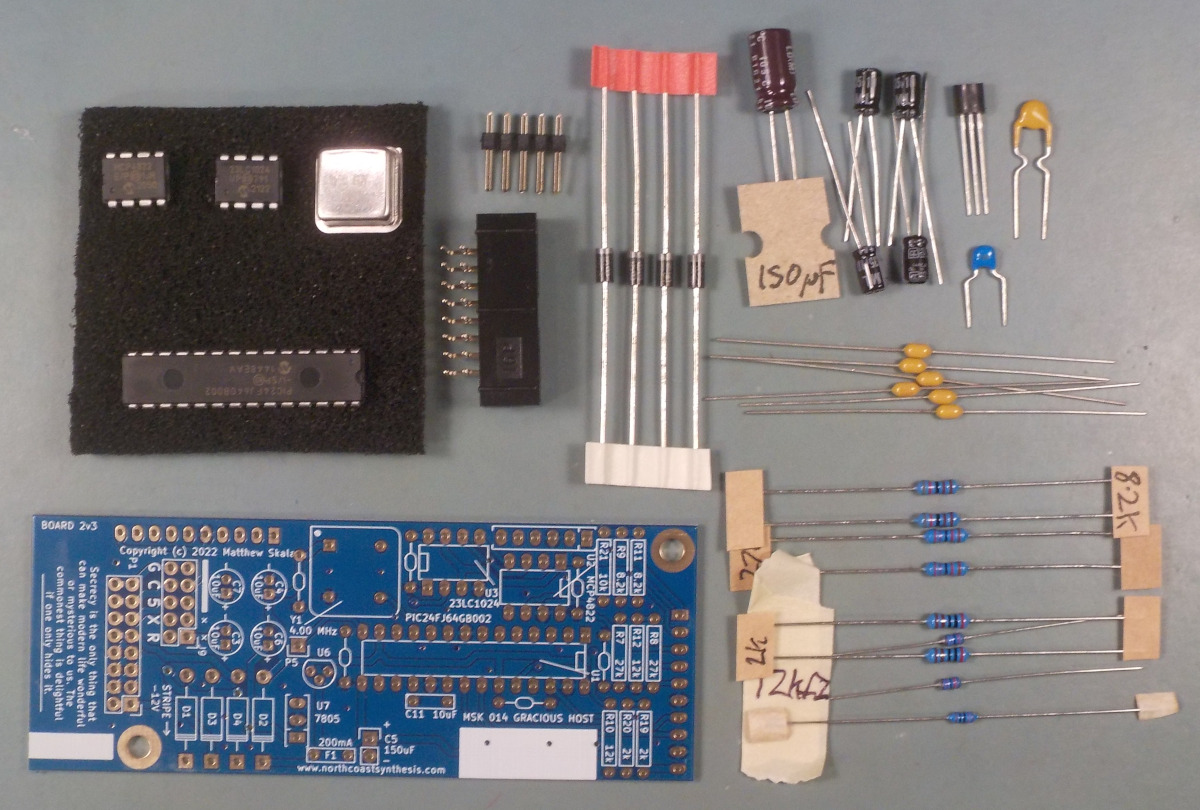
\includegraphics[width=\linewidth]{board2-parts.jpg}

\begin{table*}
{\centering
\fbox{This table is not a substitute for the text instructions.}
\vspace{\baselineskip}

\begin{tabular}{rp{1.3in}cp{3in}}
  \textbf{Qty} & \textbf{Ref} & \textbf{Value/Part No.} & \\ \hline
\input{bomdata-2.tex}
\end{tabular}\par}
\caption{Bill of Materials for assembling Board~2.  Also needed is the PCB
itself.}\label{tab:b2bom}
\end{table*}

\section{Decoupling capacitors}

The six axial ceramic 0.1$\mu$F decoupling capacitors are shown
on the board by a special symbol without their reference designators.

\nopagebreak
\noindent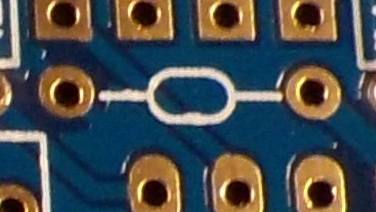
\includegraphics[width=\linewidth]{decoup-symbol.jpg}

Install these six capacitors where the symbol appears.  They are not
polarized and may be installed in either orientation.  These capacitors act
as filters for the power supplies to the ICs.  An MSK~014
kit should include ten of these capacitors, and only six are used on this
board; save the remaining four for use on Board~1.

\nopagebreak
\noindent\includegraphics[width=\linewidth]{{cap-0.1u2}.jpg}

\section{Fixed resistors}

Resistors are never polarized.  I like to install mine in a consistent
direction for cosmetic reasons, but this is electrically unnecessary.  In
this module, the fixed resistors are metal film 1\%\ type.  They usually
have blue bodies and four colour bands designating the value, plus a fifth
band for the tolerance.  The tolerance band is brown for 1\%, but note that
we may occasionally ship better-tolerance resistors in the kits than the
specifications require, if we are able to source them at a good price. 
Accordingly, I mention only the four value band colours for this type of
resistor; if you are using resistors with other codes, you are responsible
for knowing them.  Note that colour codes on metal film 1\% resistors are
often ambiguous (reading from one end or the other end may give two
different values, both plausible) and some of the colours are hard to
distinguish anyway.  If in doubt, always measure with an ohmmeter before
soldering the resistor in place.

Install the two 2k$\Omega$ (red-black-black-brown) resistors R19 and R20.
These resistors form a voltage divider that scales the USB power voltage
into a range the microcontroller can measure.

\nopagebreak
\noindent\includegraphics[width=\linewidth]{{res-2k}.jpg}

Install the two 8.2k$\Omega$ (grey-red-black-brown) resistors R9 and
R11.  These form parts of the resistor networks that scale the analog input
voltages (amplified on the other board) into the microcontroller's input
range.

\nopagebreak
\noindent\includegraphics[width=\linewidth]{{res-8.2k}.jpg}

Install the single 10k$\Omega$ (brown-black-black-red) resistor~R21.  This
is a pull-up resistor for the microcontroller's hardware reset input, which
can be overridden via the in-circuit debugging port.  There are six 10k$\Omega$
resistors in the module; reserve the other five for installing on the other
board.

\nopagebreak
\noindent\includegraphics[width=\linewidth]{{res-10k2}.jpg}

Install the two 12k$\Omega$ (brown-red-black-red) resistors R10 and R12. 
These are also parts of the analog input resistor networks.

\nopagebreak
\noindent\includegraphics[width=\linewidth]{{res-12k}.jpg}

Install the two 27k$\Omega$ (red-violet-black-red) resistors R7 and R8.
These, too, are used to scale the analog input voltages.

\nopagebreak
\noindent\includegraphics[width=\linewidth]{{res-27k}.jpg}

\section{Semiconductors}

Install the four 1N5818 or SBA130 Schottky rectifier diodes D1 through D4. 
These in general terms ensure that the different power voltages have the
proper relationships: not connected backwards, and not a lower voltage
connected while a higher voltage is disconnected; protecting the ICs and the
onboard regulators.

The diodes are polarized and it is important to install them in the right
direction.  Each diode is packaged inside a black or dark grey plastic slug
with a white or light grey stripe at one end; that end is the
\emph{cathode}.  The silkscreen markings on the board have a corresponding
stripe and the diodes should be installed with their stripes matching the
markings on the board.  The solder pads for the cathodes are also square
instead of round.  Installing the diodes backwards means they will have the
opposite of the intended protective effect.

\nopagebreak
\noindent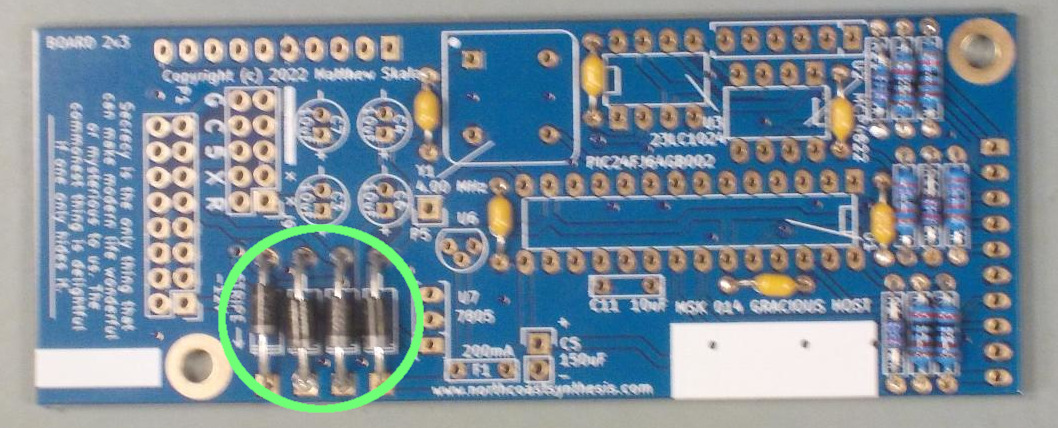
\includegraphics[width=\linewidth]{schottky.jpg}

The DIP ICs on this board are intended to be installed \emph{without
sockets}.  These ICs send and receive signals at frequencies of up to
12\,MHz (harmonics higher than that), and the microcontroller in particular
is sensitive to the stray capacitance and inductance of its connections to
other components.  Mounting it without a socket reduces those stray
reactances and improves the ability of the decoupling capacitors to keep
everything stable.  North Coast Synthesis kits for this module include some
DIP sockets, but those are meant to be used for the op amp ICs on Board~1,
not on this board.

Because these ICs are installed without sockets, it is especially important to
make sure that they are installed right way round.  If you solder one in
backwards, you will find it difficult to desolder without damage to correct
the errors.  \emph{Double check the orientation of each IC before
soldering.}  Each IC has a notch at one end, or possibly a dimple in
one corner, marking the location of Pin~1.  On the PCB silkscreen, there is
a marking indicating the location of the notch, and the pad for Pin~1 is
rectangular instead of rounded.

Install the MCP4822 DAC chip, U2.  This chip converts digital signals from
the microcontroller to analog voltages for the analog output jacks.  Make
sure that its Pin~1 marking matches that on the circuit board, pointing up,
toward what will be the top of the finished module.  Also, make sure you are
really installing the MCP4822.  It is the same size and shape as the SRAM
chip (next) and it is important not to swap them.

\nopagebreak
\noindent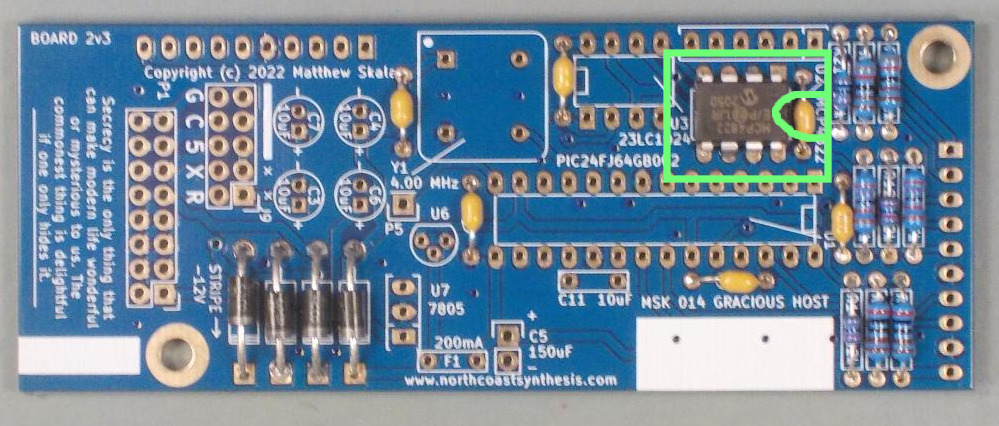
\includegraphics[width=\linewidth]{mcp4822.jpg}

Install the 23LC1024 SRAM chip, U3.  This chip provides additional memory
space for the microcontroller, which is used to buffer firmware images
during the firmware update process, as well as potentially for other purposes.
Make sure its Pin~1 marking matches that on the circuit board, pointing
\emph{down} (opposite to the previous chip) toward what will be the bottom
of the finished module.

\nopagebreak
\noindent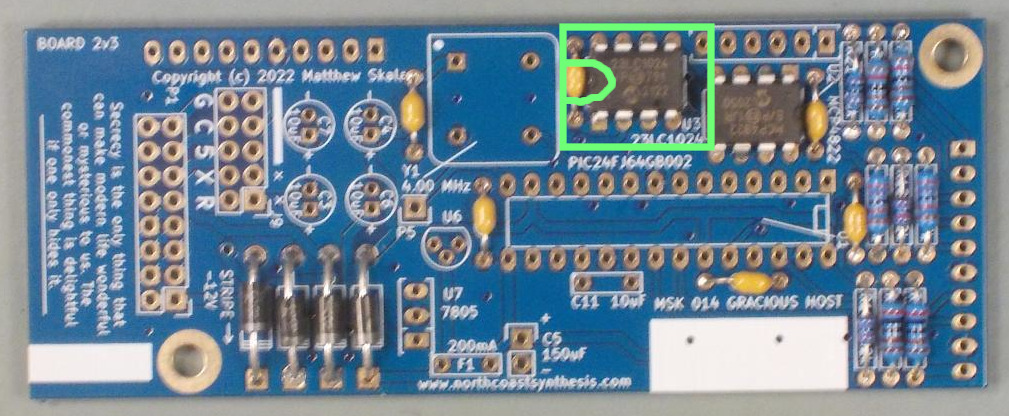
\includegraphics[width=\linewidth]{23lc1024.jpg}

Install the PIC24FJ64GB002 microcontroller chip, U1.  This chip is the heart
and brain of the module, containing a small computer, associated
peripherals, and the firmware that tells the computer what to do.  It is in
a long thin 28-pin ``skinny DIP'' package, and it may take some careful
adjustment or bending of the legs to get them all nicely fitted into the
holes on the board.  Make sure the Pin~1 marking matches that on the circuit
board, pointing up toward what will be the top of the finished module.

Note that the microcontroller chip needs to be \emph{already programmed}
before you install it; once installed, it can only be loaded with firmware
through the USB port if it already has basically functional firmware on it,
or through in-circuit debugging with the installation of an additional
header and a PIC-specific programming tool.  Chips shipped in North Coast
Synthesis kits come pre-programmed.

\nopagebreak
\noindent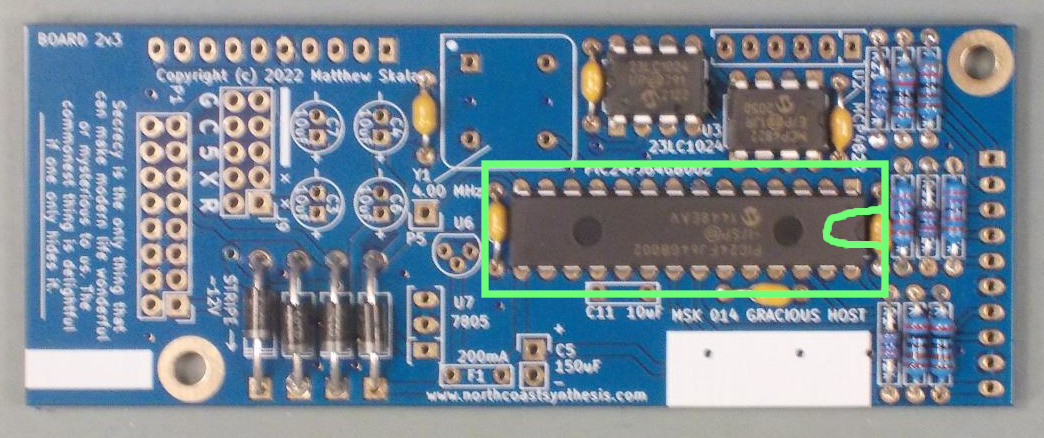
\includegraphics[width=\linewidth]{pic24fj64gb002.jpg}

Install the 4.000\,MHz clock oscillator module Y1.  This is a hybrid device
including an oscillator chip, a quartz crystal, and some support components,
all inside a sealed metal can.  It provides a stable and accurate reference
frequency which will be multiplied and divided by the microcontroller chip
to provide timing references for all parts of the Gracious Host.

The oscillator mounts in four holes arranged in a square pattern (basically
the four corner holes of an 8-pin DIP footprint) and that makes orientation
important.  It can fit into the board in four different orientations, only
one of which is correct.  One corner of the oscillator will be marked,
probably with a sharp point on the can where the other three corners are
rounded, and a dot etched into the upper surface near the special corner. 
That corner represents Pin~1.  The sharp corner and dot are shown on the PCB
silkscreen and the oscillator should be mounted to match its markings with
the silkscreen.  The solder pad for Pin~1 is also square, whereas the other
three are circular.

\nopagebreak
\noindent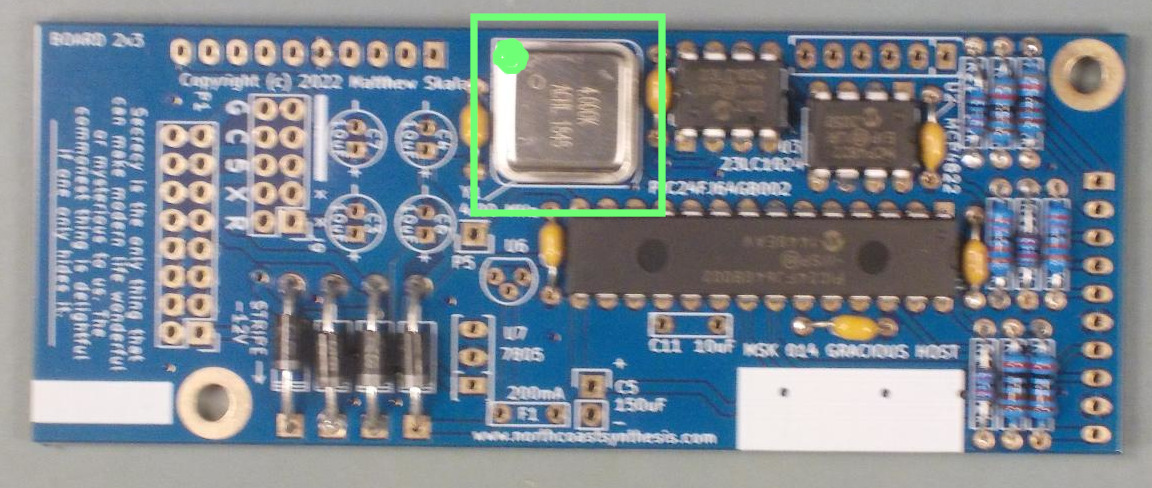
\includegraphics[width=\linewidth]{crystal.jpg}

Install the MCP1700-3302 voltage regulator chip, U6.  This is an LDO (low
drop out) regulator that reduces the $+$5V Eurorack power supply to $+$3.3V
for the digital chips.  The PIC24 actually runs on $+$2.55V internally, and
has a built-in regulator of its own to extract that from the $+$3.3V input.

The voltage regulator uses a TO-92 package, which is a small epoxy
pill like a transistor package.  The package has one flat side, and it
should be installed with that flat side matching the flat side shown in the
PCB silkscreen, facing the oscillator module.  Bend the middle lead of the
TO-92 backward to match the triangular hole pattern on the board.

\nopagebreak
\noindent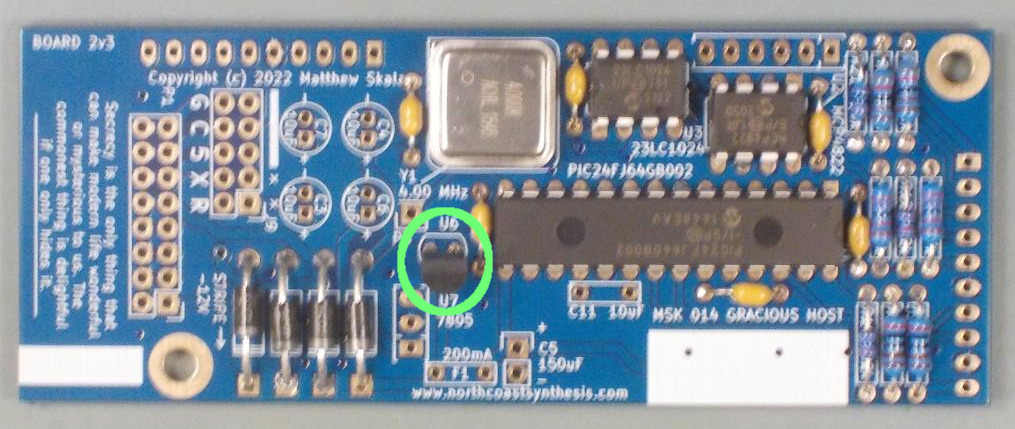
\includegraphics[width=\linewidth]{mcp1700-3302.jpg}

There are three pads on this board labelled ``U7 7805,'' near the LDO
regulator just installed, for installing an optional
$+$5V regulator.  See the comments in the general notes chapter of this
manual for more information about installing this regulator.  In most
builds, it is not recommended.

\section{Capacitors and fuse}

Install the four 10$\mu$F aluminum electrolytic capacitors C3, C4, C6, and
C7.  These are used for general filtering of the main power supplies:
$\pm$12V, $+$5V, and $+$3.3V, mostly for relatively low frequency noise.
They are polarized components and they may explode if installed backwards. 
Each one will be marked on its casing with a stripe and minus signs to
indicate the negative lead; the positive lead will probably also be longer. 
These clues should be matched with the markings on the PCB: plus and minus
symbols in the silkscreen and a square solder pad for the positive (long)
lead.

\nopagebreak
\noindent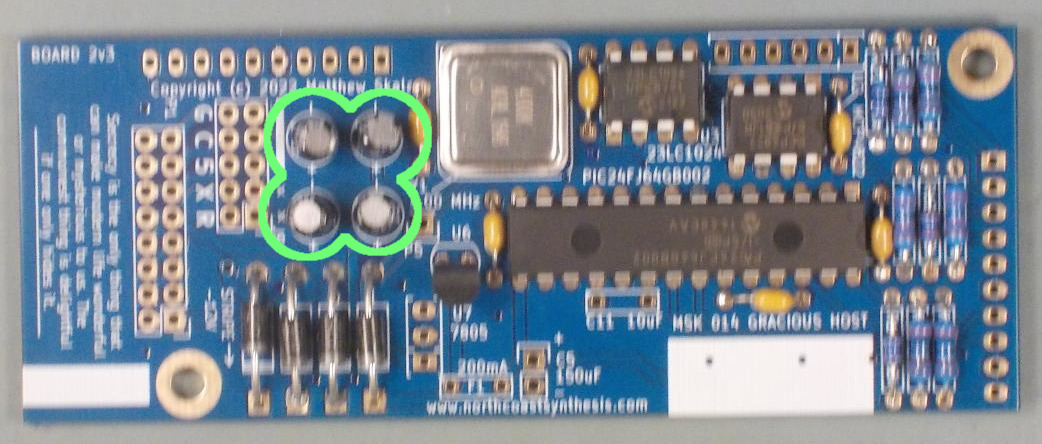
\includegraphics[width=\linewidth]{cap-10u.jpg}

Install the 10$\mu$F ceramic capacitor C11.  This is a special
high-frequency filter for the PIC24's built-in core voltage regulator.  Be
sure not to confuse this capacitor with the other ceramic capacitors; it
is about the same physical size as the 100pF capacitors used on the other
board, but electrically it is very much bigger than them.  It is not
polarized.

\nopagebreak
\noindent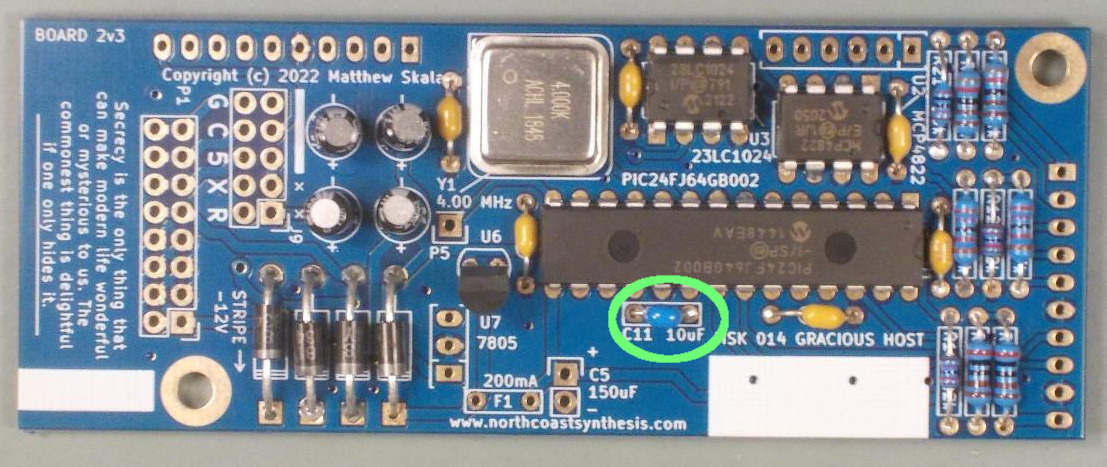
\includegraphics[width=\linewidth]{cap-10ucer.jpg}

Install the 200\,mA ``polyfuse'' F1.  This device looks like a ceramic disc
capacitor with kinks in the leads, but is actually a special
kind of temperature-sensitive resistor.  It serves to protect the USB power
supply line from short circuits.  It is unpolarized.  Install it in the pads
labelled F1.  If you bend the leads to keep it from sticking out too far,
then be careful not to leave it resting in direct contact with other
components.

\nopagebreak
\noindent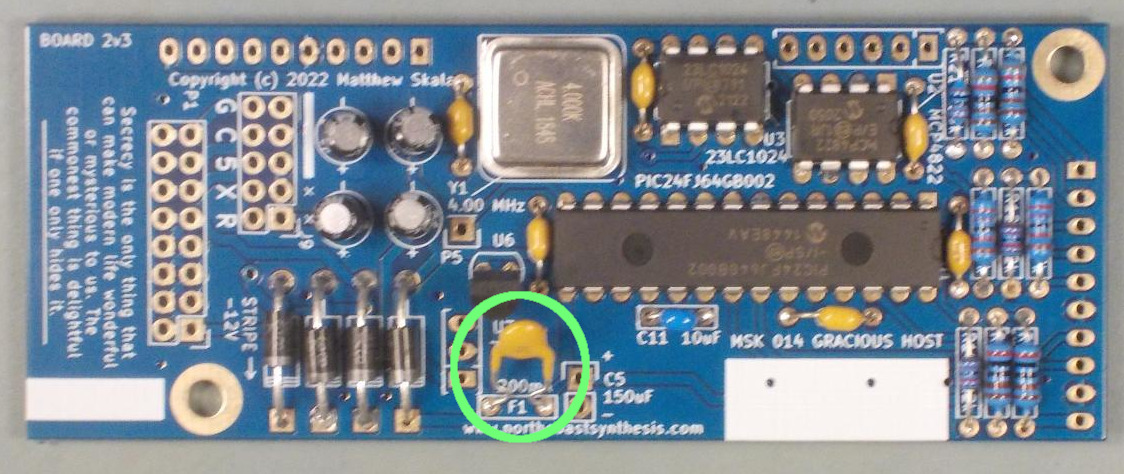
\includegraphics[width=\linewidth]{polyfuse.jpg}

Install the 150$\mu$F aluminum electrolytic capacitor C5.  This capacitor
provides a substantial reservoir of charge for buffering transients as USB
devices are plugged and unplugged.  It looks like a physically larger
version of the smaller aluminum electrolytics installed earlier, and like
them, it is polarized and marked with a stripe on the body for negative and
a longer lead for positive.  The two pads on the board are labelled $+$ and
$-$ to indicate which is which, and the $+$ pad is square.

You will probably find it most convenient to lay the 150$\mu$F capacitor on
its side on the board, with the leads bent down to go into the pads.  You
may need to secure it to the board with putty or tape to hold it in place
while soldering, but once soldered it should be reasonably rugged.

\nopagebreak
\noindent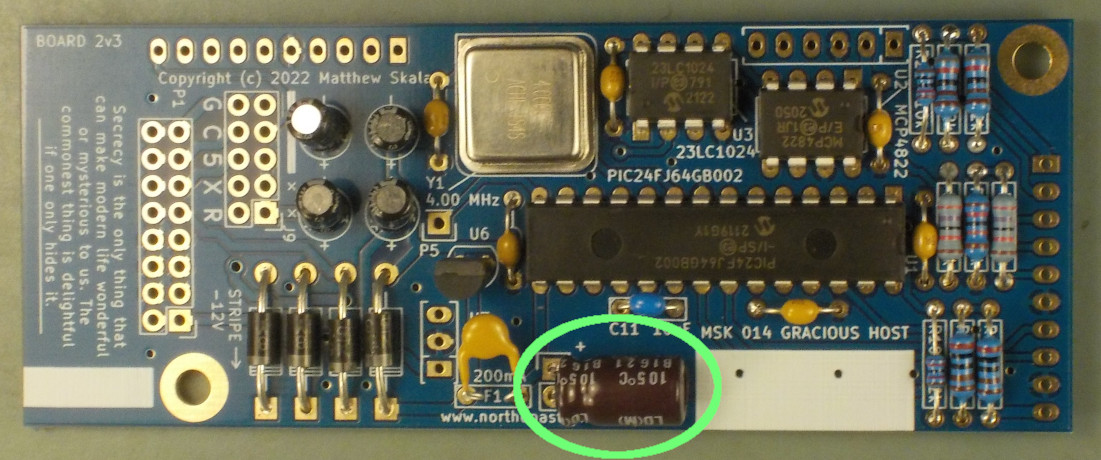
\includegraphics[width=\linewidth]{cap-150u.jpg}

\section{Header connectors}

Install the 2$\times$5-pin header connector J9.  This connector is used with
configuration jumpers to select whether the module should or should not
connect to the Eurorack CV/gate bus, and the source of the module's $+$5V
power.  Try to install it snugly against the board, not tilted at an angle. 
Use tape or putty to hold it in place, solder one pin, then check that it is
straight before you solder the other pins.

\nopagebreak
\noindent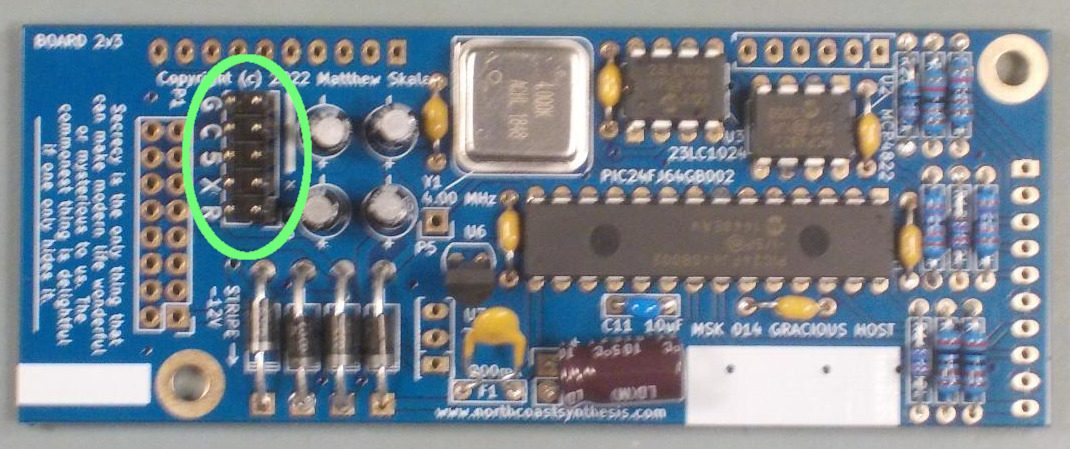
\includegraphics[width=\linewidth]{jumperblock.jpg}

Install the 2$\times$8-pin shrouded power connector P1.  This is used for
connecting the module to the Eurorack bus, for power and CV/gate output.  As
with the jumper block, it may be useful to solder just one pin and check the
angle before soldering the rest, though the much larger body of this
connector will probably make it easier to keep flat on the board.

\nopagebreak
\noindent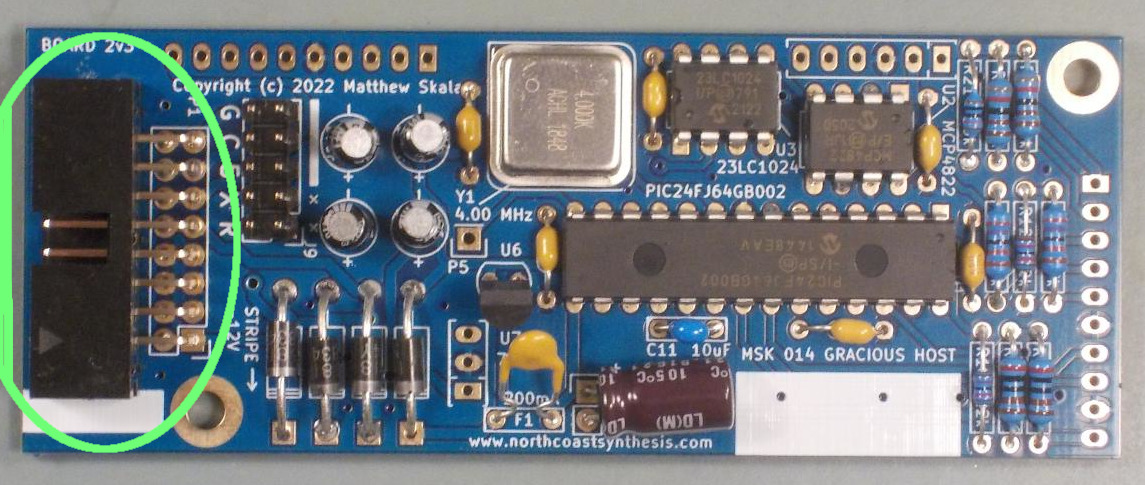
\includegraphics[width=\linewidth]{power.jpg}

The board-to-board header connectors P2 and P3 will be installed on this
board later, during the build of Board~1.  There is also a footprint on this
board for a header connector named P4, which is for in-circuit debugging and
not installed in a standard build.

In between completed boards is a good time to take a break.
